\chapter{Messergebnisse}

Dieses Kapitel be\-han\-delt die Mess\-er\-geb\-nis\-se, welche mit dem zu\-vor be\-schrie\-be\-nen System erzielt wurden. Dabei wird von verschiedenen Sze\-narien aus\-ge\-gang\-en, welche die jeweiligen Vor- und Nach\-teile der zwei Sy\-stem\-e zum Ausdruck bringen sollen. 

\section{Laborumgebung}

Alle Mes\-ser\-ge\-bnis\-se stam\-men aus einer Labor\-umgebung, mit folgenden Ei\-gen\-schaf\-ten:

\begin{itemize}
\item Alle Testrechner, Server wie Client, besitzen folgende Hardware:
\begin{itemize}
\item Prozessor: Intel Xeon CPU X3450, 8 x 2.67Ghz
\item Speicher: RAM 8GB
\item Netzwerkkarte: Intel 82578DM Gigabit Network Card
\end{itemize}
\item Folgende Betriebssysteme wurden während den Messungen verwendet:
\begin{itemize}
\item Server: Ubuntu, Version 11.10
\item Auf beiden Clients: Fedora Linux, Release 16
\end{itemize}
\item Die Netzwerkinfrastruktur im Laborraum ist kaum belastet, nur durch den gebräuchlichen Leerlaufverkehr(\gls{STP}, \gls{ARP} usw.)
\item Die Hardware-Ressourcen der Rechner, auf welchen die Applikation getestet wird, sind ausschliesslich nur durch die Applikation belegt und durch einzelne, übliche Prozesse vom  Betriebsystem.
\end{itemize}

\section{Testvorgaben}
Die in dieser Arbeit ausgewiesenen Zahlen wurden alle in der La\-bor\-um\-gebung ge\-mes\-sen. Dabei wurde für jeden Test\-Case die An\-zahl der Clients schritt\-weise von zwei bis acht Clients erhöht. Jeder Test\-lauf mit der gleichen Anzahl Clients, wurde drei Mal durchgeführt, um einen exakten Mittel\-wert der Er\-geb\-nis\-se aus\-weisen zu können. Drei Test\-durchläufe pro Szenario und Clientanzahl wurden aufgrund der sehr dicht beieinander liegenden Er\-geb\-nis\-se der Testdurchläufe als genügend eingestuft. Wären die einzelnen Ergebnisse der Durchläufe extrem unterschiedlich ausgefallen, hätten fünf oder mehr Durchläufe stattfinden müssen.

\section{Testergebnisse}
In den folgenden Kapiteln werden die getesteten Szenarios und deren Ergebnisse gezeigt. \\
Die in der Legende der Tabellen beschriebenen Funktionen lassen sich wie folgt erklären:
\begin{description}
\item[setBalance()] Die durchschnittliche Zeit, welche benötigt wird, um einen schreibenden Zugriff zu tätigen.
\item[getBalance()] Die durchschnittliche Dauer, um einen lesenden Zugriff zu tätigen.
\item[Number of Conflict] Anzahl Konflikte, welche während des Testlaufs aufgetreten sind.
\item[Total Time(with Delays)] Beschreibt die Zeit, welche gebraucht wurde, um das gesamte Szenario, inklusive Konfliktbewältigung und konfigurierte Verzögerung, durchzuspielen.
\item[Pure Operation Time] Die für das Durchspielen des Szenarios benötigte Zeit, ohne die konfigurierten Verzögerungen.
\end{description}


\subsection{Nur lesende Clients}
\subsubsection{Szenario Code}
Dieser TestCase sieht folgendermassen aus:
\begin{lstlisting}[language=XML, breaklines=true]
<?xml version='1.0' encoding='UTF-8'?>
<TestRun>
  <TestCase
    ClientSystemUnderTest="ch.hsr.objectCaching.rmiWithCacheClient.RMIwithCacheClientSystem"
    ServerSystemUnderTest="ch.hsr.objectCaching.rmiWithCacheServer.RMIWithCacheServerSystem">
    <Account balance="1"></Account>
      <Scenario id="1">
        <ActionSequence>
          <Read count="250"></Read>
	</ActionSequence>
      </Scenario>
  </TestCase>
</TestRun>
\end{lstlisting}

\subsubsection{Szenariobeschreibung}
Bei diesem Testcase führen alle Clients die gleichen Operationen aus. Alle Clients lesen das Objekt auf dem Server genau 250 Mal. Das Account-Objekt wird mit dem Wert "'1"' initialisiert, welcher bis zum Schluss unverändert bleiben wird. 

Dieses Testszenario soll zeigen, welches der beiden System bei nur Lesezugriffen besser skaliert.

\subsubsection{Ergebnisse System ohne Cache}

Die folgende Tabelle stellt die Mess\-er\-geb\-nis\-se des Sys\-tems ohne Cache dar:  \newline


\resizebox{6cm}{!} {
\begin{tabular*}{6.5cm}[]{l l l l l l}
Legende&2 Clients&3 Clients&4 Clients&5 Clients\\
\cline{1-5}
setBalance[ms]&0&0&0&0\\
getBalance[ms]&86.182&89.502273&91.313&94.490998\\
Number of Conflict&0&0&0&0\\
TotalTime(with Delays)[ms]&21546.54&22376.494&22829.21&23623.678\\
PureOperationTime[ms]&21545.686&22375.568&22828.264&23622.749\\
\end{tabular*} }
\newline
\newline

\resizebox{6cm}{!} {
\begin{tabular*}{6.5cm}[]{l l l l}
Legende&6 Clients&7 Clients&8 Clients\\
\cline{1-4}
setBalance[ms]&0&0&0\\
getBalance[ms]&98.381525&105.14788&120.2947\\
Number of Conflict&0&0&0\\
TotalTime(with Delays)[ms]&24596.331&26287.93&30074.669\\
Pure Operation Time[ms]&24595.381&26286.969&30073.691\\
\end{tabular*} } \newline

Diese Zahlen sind Durch\-schnitt\-swer\-te von drei Messungen. Die genauen Mess\-daten können im Anhang gefunden werden. Die folgende Grafik zeigt den Verlauf des Zeit\-auf\-wandes mit einer steigenden Anzahl Clients von zwei bis acht Clients:
\begin{figure}[H]
\begin{center}
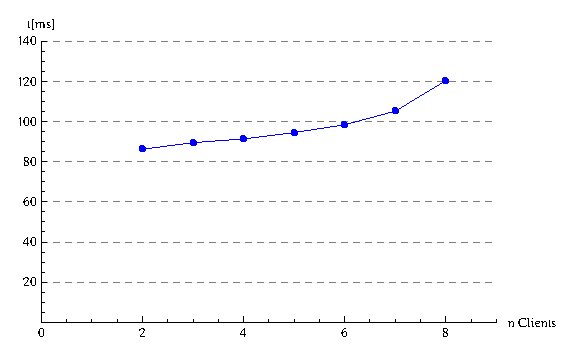
\includegraphics[width=\textwidth]{images_MessErgebnisse/getBalance_RMI.eps}
\caption{\texttt{getBalance()}-Zeitaufwand, System ohne Cache(nur lesende Zugriffe)}
\end{center}
\end{figure}
Es wird schnell ersichtlich, dass das System mit einer steigenden Anzahl Clients langsamer wird. Dies erscheint durchaus logisch, da jeder \texttt{get\-Balance()}-Aufruf an den Server gesendet wird. Wird der Server nun von mehreren Clients angefragt, verschlechtern sich auch dessen Antwortzeiten, was eine Verlangsamung des Aufrufs zur Folge hat.

\subsubsection{Ergebnisse System mit Cache}

In der folgenden Tabelle werden die Messdaten des Cache-Systems dar\-ge\-stellt: \newline


\resizebox{6cm}{!} {
\begin{tabular*}{6.5cm}[]{l l l l l l}
Legende&2 Clients&3 Clients&4 Clients&5 Clients\\
\cline{1-5}
setBalance[ms]&0&0&0&0\\
getBalance[ms]&0.288&0.287&0.285&0.298\\
Number of Conflict&0&0&0&0\\
TotalTime(with Delays)[ms]&73.087&72.581&72.039&75.422\\
PureOperationTime[ms]&72.249&71.855&71.304&74.603\\
\end{tabular*} }
\newline
\newline

\resizebox{6cm}{!} {
\begin{tabular*}{6.5cm}[]{l l l l}
Legende&6 Clients&7 Clients&8 Clients\\
\cline{1-4}
setBalance[ms]&0&0&0\\
getBalance[ms]&0.3011&0.3201&0.281\\
Number of Conflict&0&0&0\\
TotalTime(with Delays)[ms]&76.014&80.838&71.001\\
Pure Operation Time[ms]&75.289&80.041&70.262\\
\end{tabular*} } \newline

Diese Zahlen sind wiederum Durch\-schnitts\-wer\-te.  In der folgenden Grafik werden die durch\-schnitt\-li\-chen Zeiten der \texttt{getBalance()}-Methode in Ab\-hän\-gig\-keit der Anzahl Clients aus\-ge\-geben:

\begin{figure}[H]
\begin{center}
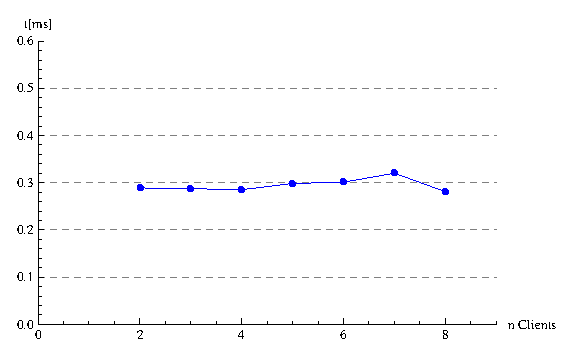
\includegraphics[width=\textwidth]{images_MessErgebnisse/getBalance_03ms.eps}
\end{center}
\caption{\texttt{getBalance()}-Zeitaufwand, System mit Cache(nur lesende Zugriffe)}
\end{figure}

Damit die Grafik einen Sinn ergibt, mussten die Zeiten auf der Y-Achse an\-ge\-passt werden. Hätte man die Skala aus dem RMI-Only-System über\-nom\-men, wäre auf der Grafik nur eine Linie er\-sicht\-lich. Es muss dennoch bemerkt werden, dass bei dieser Grafik die Skala auf der Y-Achse extrem klein ist und Mess\-un\-ter\-schiede, wenn auch nur mi\-ni\-male, in dieser Grafik stark zum Tragen kommen. Ein Ver\-gleich mit der vor\-her\-gehenden Grafik des Systems ohne Cache ist also mit Vorsicht zu geniessen.

Aus der Grafik wird ersichtlich, dass bei nur lesenden Zu\-griffen das System perfekt skaliert. Die Werte betragen circa alle, egal wieviele Clients beteiligt sind, 0.3ms. 


\subsubsection{Interpretation}

Vergleicht man die Messergebnisse der zwei Systeme miteinander, fallen zwei Merkmale auf:
\begin{itemize}
\item Jeder einzelne getBalance-Aufruf dauert beim System ohne Cache extrem viel länger
\item Das Cache-System skaliert viel besser als das System ohne Cache
\end{itemize}

Da jeder getBalance-Aufruf zum Server, das heisst über das Netzwerk,
übertragen werden muss, ist es logisch, dass das System im
Durchschnitt viel langsamer ist. Beim Cache-System wird nur der erste
Aufruf zum Server übertragen, alle folgenden Aufrufe werden lokal aus
dem Cache beantwortet. Dies erklärt den enormen
Geschwindigkeitsvorteil des Cache-Systems bei jedem einzelnen Aufruf.

Weiter skaliert das Cache-System bei diesem Testcase um einiges besser. Dadurch, dass bei steigender Anzahl Clients auch immer mehr Clients ein Update erhalten müssen, hätte man auch eine leichte Steigung der Messwerte beim Cache-System erwarten können. Da die Werte aber so klein sind und die Messmethode mit der in Java implementierten Funktion \texttt{nanoTime()} gemacht wurde, können kleine Ungenauigkeiten in diesem Bereich nicht ganz ausgeschlossen werden. Es bleibt auf jeden Fall zu beachten, dass das Cache-System wunderbar skaliert. Vermutlich hätte das Szenario mit einer Vielzahl der Clients durchgeführt werden können, ohne grosse Geschwindigkeitseinbussen in Kauf nehmen zu müssen.

Auf der anderen Seite skaliert das System ohne Cache weitaus schlechter. Bei der Erhöhung der Clients von vier bis acht, also rund eine Verdopplung der Clients, wächst die durchschnittliche Zeit zum Ausführen der getBalance-Methode um etwa 30ms. Dies entspricht einem Drittel der Zeit, welche ein \texttt{getBalance()}-Aufruf bei vier Clients benötigt. Würde man die An\-zahl Cli\-ents noch verdoppeln oder sogar verdreifachen, würde die benötigte Zeit zum Ausführen der \texttt{getBalance()}-Methode vermutlich bald eine Schmerzgrenze der Wartezeiten durchbrechen.

\subsection{Ein schreibender, mehrere lesende Clients}
\subsubsection{Szenario Code}
Das Szenario ist wie folgt aufgebaut:
\begin{lstlisting}[language=XML, breaklines=true]
<?xml version='1.0' encoding='UTF-8'?>
<TestRun>
  <TestCase
    ClientSystemUnderTest="ch.hsr.objectCaching.rmiWithCacheClient.RMIwithCacheClientSystem"
    ServerSystemUnderTest="ch.hsr.objectCaching.rmiWithCacheServer.RMIWithCacheServerSystem">
      <Account balance="1"></Account>
        <Scenario id="1">
	  <ActionSequence>
	    <Increment count="900" delay="0" factor="1.1"></Increment>
	  </ActionSequence>
	</Scenario>
	<Scenario id="2">
	  <ActionSequence>
	    <Read count="3000" delay="100"></Read>
	  </ActionSequence>
	</Scenario>
	<Scenario id="3">
	  <ActionSequence>
	    <Read count="3000" delay="100"></Read>
	  </ActionSequence>
	</Scenario>
	...
	...
\end{lstlisting}

Das Szenario ist nicht abschliessend dargestellt, da sich nun bis zum Szenario mit der Id acht, die Szenariodefinitionen wiederholen. Der erste in der Clientliste eingetragene Client, wird immer den schreibenden Auftrag bekommen. Die anderen eins bis sieben Clients werden nur den Auftrag bekommen zu lesen. \newline
Für diesen Testcase wurde bei der Leseaktion extra noch ein Delay eingebaut. Die Clients müssen so lange lesen, wie der schreibende Client am Arbeiten ist. Wären die lesenden Clients schon vor dem schreibenden Client fertig, würden sie sich herunterfahren und keine Updates mehr erhalten. Dies würde den Testcase verfälschen und somit nutzlos machen. Damit nun keine Million Reads angegeben werden mussten, wurde ein Delay eingebaut, damit die Clients lange genug aktiv bleiben. 
\subsubsection{Szenariobeschreibung}
In diesem Szenario geht es darum, dass nur ein Client den Balance-Wert erhöht und alle anderen Clients diesen Wert lesen. Es soll daher gezeigt werden, wie stark sich die Updates, welche beim System mit Cache versendet werden, auf die Performance des Systems auswirken. Weiter ist von Interesse, wie stark die Performance bei einer steigenden Anzahl Clients, daher einer steigenden Anzahl Updates, tangiert wird. \\

Die folgende Auswertung der Mess\-resultate be\-schränkt sich auf den schrei\-ben\-den Client. Es soll unter\-sucht werden, ob und wie stark sich eine stei\-gen\-de Anzahl le\-sen\-der Clients auf die Schreib\-dauer eines Clients auswirkt. 

\subsubsection{Ergebnisse System ohne Cache}

Die Messwerte des schreibenden Clients sehen wie folgt aus: \newline


\resizebox{6cm}{!} {
\begin{tabular*}{6.5cm}[]{l l l l l l}
Legende&2 Clients&3 Clients&4 Clients&5 Clients\\
\cline{1-5}
setBalance[ms]&79.870&79.951&79.821&79.858\\
getBalance[ms]&80.124&80.140&80.114&80.142\\
Number of Conflict&0&0&0&0\\
TotalTime(with Delays)[ms]&80003.557&80051.669&79973.797&80006.288\\
PureOperationTime[ms]&79997.736&80045.911&79968.060&80000.453\\
\end{tabular*} }
\newline
\newline

\resizebox{6cm}{!} {
\begin{tabular*}{6.5cm}[]{l l l l}
Legende&6 Clients&7 Clients&8 Clients\\
\cline{1-4}
setBalance[ms]&79.914&79.876&80.081\\
getBalance[ms]&80.133&80.124&80.201\\
Number of Conflict&0&0&0\\
TotalTime(with Delays)[ms]&80029.782&80006.137&80105.944\\
Pure Operation Time[ms]&80024.009&80000.355&80100.144\\
\end{tabular*} } \newline

Die Ergebnisse der \texttt{setBalance()}-Aurufe werden in dieser Abbildung grafisch dargestellt:

\begin{figure}[H]
\begin{center}
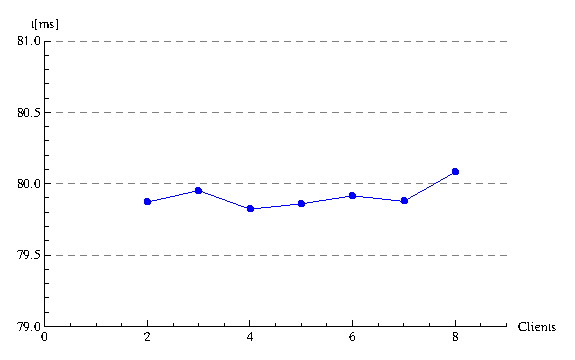
\includegraphics[width=\textwidth]{images_MessErgebnisse/incrementAndReadRMI.eps}
\end{center}
\caption{\texttt{setBalance()}-Zeitaufwand, System ohne Cache(lesende/schreibende Zugriffe)}
\end{figure}

Das System ohne Cache skaliert sehr gut. Die Werte für einen sch\-rei\-ben\-den Zugriff bleiben stabil.

\subsubsection{Ergebnisse System mit Cache}

Folgende Tabelle zeigt die Messer\-gebnisse des schreibenden Clients mit dem Cache-System: \newline


\resizebox{6cm}{!} {
\begin{tabular*}{6.5cm}[]{l l l l l l}
Legende&2 Clients&3 Clients&4 Clients&5 Clients\\
\cline{1-5}
setBalance[ms]&88.7521&88.789&88.603&88.620\\
getBalance[ms]&0.1837&0.184&0.185&0.184\\
Number of Conflict&0&0&0&0\\
TotalTime(with Delays)[ms]&80144.642&80149.519&79982.694&80025.973\\
PureOperationTime[ms]&80131.176&80136.188&79969.438&80012.822\\
\end{tabular*} }
\newline
\newline

\resizebox{6cm}{!} {
\begin{tabular*}{6.5cm}[]{l l l l}
Legende&6 Clients&7 Clients&8 Clients\\
\cline{1-4}
setBalance[ms]&88.655&88.766&88.920\\
getBalance[ms]&0.189&0.180&0.192\\
Number of Conflict&0&0&0\\
TotalTime(with Delays)[ms]&80003.756&80093.180&80244.857\\
Pure Operation Time[ms]&79990.542&80081.593&80231.319\\
\end{tabular*} } \newline

In der folgenden Grafik ist der Verlauf der Messwerte der \texttt{setBalance()}-Aufrufe des schreibenden Clients zu sehen:
\begin{figure}[H]
\begin{center}
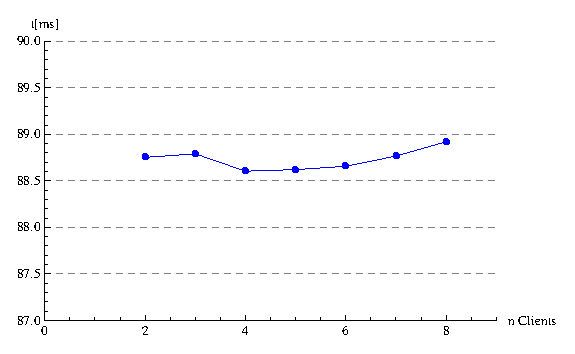
\includegraphics[width=\textwidth]{images_MessErgebnisse/incrementAndReadCache.eps}
\end{center}
\caption{\texttt{setBalance()}-Zeitaufwand, System mit Cache(lesende/schreibende Zugriffe)}
\end{figure}

Das System mit Cache skaliert sehr gut. Die gemessenen Zeiten der \texttt{set\-Balance()}-Aufrufe steigen auch mit zunehmenden Clients nicht an.

\subsubsection{Interpretation}

Aufgrund der Messergebnisse kann geschlossen werden, dass die Updates des Servers keinen Einfluss auf die Performance der Systeme hat. Da die Ergebnisse stabil bleiben, egal wie viele Clients beteiligt sind, kann eine starke Beeinträchtigung des Servers und der Clients ausgeschlossen werden. Es ist daher anzunehmen, dass die Performancewerte weiter stabil bleiben würden, auch wenn die Anzahl Clients um ein Vielfaches steigen würde.\\

Auch das System ohne Cache skaliert sehr gut. Die Werte der \texttt{set\-Balance()}-Aufrufe sind stabil und liegen alle nahe beieinander. Aufgrund der Zahlen ist ersichtlich, dass der Server die Anfragen schnell und zuverlässig abfertigen kann. Trotz der Steigerung der Clients, konnten keine Performanceverluste ausgemacht werden. Dies lässt darauf schliessen, dass der Server durch die Anfragen nicht stark belastet wurde.\\

Abschliessend lässt sich zu diesem Testcase sagen, dass weder das eine, noch das andere System abfällt. Beide arbeiten stabil und fehlerlos und wenn nur die \texttt{setBalance()}-Werte betrachtet werden, auch fast gleich schnell. Die langsamen \texttt{getBalance()}-Aufrufe bleiben ein grosser Nachteil des Systems ohne Cache. 

\subsection{Nur schreibende Clients}
\subsubsection{Szenario Code}
Der XML-Code, welcher dieses Szenario beschreibt, ist hier zu sehen:
\begin{lstlisting}[language=XML, breaklines=true]
<?xml version='1.0' encoding='UTF-8'?>
<TestRun>
  <TestCase
    ClientSystemUnderTest="ch.hsr.objectCaching.rmiWithCacheClient.RMIwithCacheClientSystem"
    ServerSystemUnderTest="ch.hsr.objectCaching.rmiWithCacheServer.RMIWithCacheServerSystem">
    <Account balance="1"></Account>
      <Scenario id="1">
	<ActionSequence>
	  <Increment count="1000" delay="0" factor="1.1"></Increment>
	</ActionSequence>
      </Scenario>
  </TestCase>
</TestRun>
\end{lstlisting}
\subsubsection{Szenariobeschreibung}
In diesem Testcase führt jeder Client 1'000 Mal ein Increment auf den Balance-Wert aus. Ein Increment bedeutet den Wert zu lesen und ihn dann mit einem Faktor multipliziert wieder zu schreiben. 

Ziel dieses Szenarios ist zu zeigen, wie sich die zwei Systeme bei permanentem Schreibzugriff verhalten. Dieses Szenario stellt eine enorme Belastung für den Server dar, da er mit Anfragen geradezu bombadiert wird. Durch die vielen Anfragen wird das System auch eine längere Zeit arbeiten müssen und so zum Vorschein bringen, ob es stabil und über längere Zeit sicher und fehlerlos läuft. 

Bei steigender Anzahl Clients, wird es auch mehr Schreibzugriffe auf den Server geben. Dies führt zu mehr Netzwerkverkehr und vor allem zu mehr Last auf dem Server, welcher alle Anfragen beantworten muss. Es soll ersichtlich werden, welches Serversystem mit dieser erhöhten Last besser umgehen kann.

Ein weiteres Ziel dieses Szenarios ist zu testen, ob und wie stark sich die unterschiedliche Implementierung des Concurrency-Control Mechanismusses auf die Performance auswirkt. Das System mit Cache verfügt über zwei Mechanismen, einer im Cache und der zweite auf dem Server. Beim System ohne Cache ist nur ein Concurrency-Control auf dem Server implementiert. 

\subsubsection{Ergebnisse System ohne Cache}

Die Messerwerte des RMI-Only-Systems: \newline


\resizebox{6cm}{!} {
\begin{tabular*}{6.5cm}[]{l l l l l l}
Legende&2 Clients&3 Clients&4 Clients&5 Clients\\
\cline{1-5}
setBalance[ms]&80.119789&80.245101&80.301833&80.341942\\
getBalance[ms]&79.877294&79.774314&79.754846&79.772539\\
Number of Conflict&500&1208.44&1661.33&2367.0667\\
TotalTime(with Delays)[ms]&240019.37&353423&415639.29&539152.12\\
PureOperationTime[ms]&240003.25&353400.43&425985.248&539121.21\\
\end{tabular*} }
\newline
\newline

\resizebox{6cm}{!} {
\begin{tabular*}{6.5cm}[]{l l l l}
Legende&6 Clients&7 Clients&8 Clients\\
\cline{1-4}
setBalance[ms]&80.308807&80.276285&80.30729\\
getBalance[ms]&79.700759&79.73294&79.710938\\
Number of Conflict&2902.2778&3242.90&4371.66\\
TotalTime(with Delays)[ms]&624456.67&678747.88&859636.25\\
Pure Operation Time[ms]&624422.52&678712.13&859593.5\\
\end{tabular*} } \newline

Die nächste Grafik zeigt die Messdaten der \texttt{setBalance()}-Methode:
\begin{figure}[H]
\begin{center}
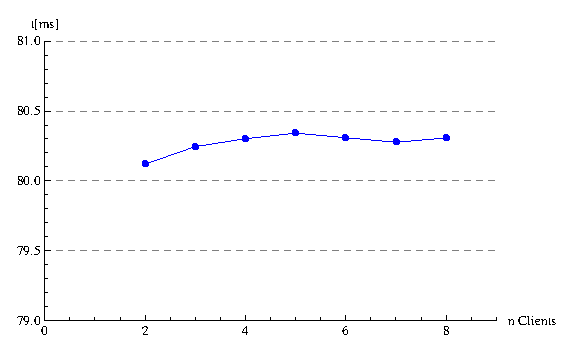
\includegraphics[width=\textwidth]{images_MessErgebnisse/incrementRMISetBalance.eps}
\end{center}
\caption{\texttt{setBalance()}-Zeitaufwand, System ohne Cache(nur schreibende Zugriffe)}
\end{figure}

Die Werte der \texttt{setBalance()}-Aufrufe bleiben stabil bei 80ms. Die Anzahl der Konflikte steigt mit der steigenden Anzahl Clients.\\

Die Latenz von etwa 80ms kommt auf Grund des Netzwerks zustande. Wie in den ausgewiesenen Zahlen der vorhergehenden Testcases gesehen werden konnte, benötigt der durchschnittliche Aufruf über das Netzwerk etwa 80ms.\\

Folgende Grafik stellt die durchschnittliche Anzahl Konflikte dar:

\begin{figure}[H]
\begin{center}
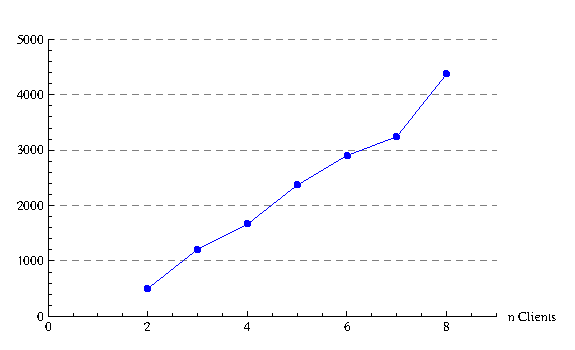
\includegraphics[width=\textwidth]{images_MessErgebnisse/incrementRMIKonfliktzahl.eps}
\end{center}
\caption{Anzahl Konflikte, System ohne Cache(nur schreibende Zugriffe)}
\end{figure}

Die Grafik zeigt eine lineare steigende Gerade. Jeder dazukommende Client verursacht im ganzen System circa 1000 Konflikte mehr, bei einer Operationsanzahl von 1000 Operationen. \\

Die "'Pure Operation Time"' ist die Summe der Zeiten aller ausgeführten Operationen:

\begin{figure}[H]
\begin{center}
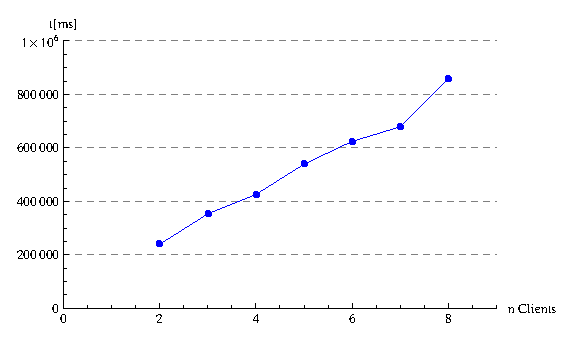
\includegraphics[width=\textwidth]{images_MessErgebnisse/incrementRMIPureOperationTime.eps}
\end{center}
\caption{Pure Operation Time System ohne Cache(nur schreibende Zugriffe)}
\end{figure}

Obwohl die \texttt{setBalance()}-Aufrufe immer konstant gleich viel Zeit be\-nö\-t\-i\-gen, steigt durch die Konfliktanzahl die "'Pure Operation Time"' an. Da die Gerade der \texttt{setBalance()}-Methode keine Steigung aufweist und die Konfliktanzahl linear steigt, ist bei der "'Pure Operation Time"' auch eine linear steigende Gerade zu sehen. Der Zusammenhang wird hier noch einmal dargelegt:
\begin{itemize}
\item Bei steigender Clientanzahl, steigt auch die Anzahl der Konflikte.
\item Für jeden Konflikt muss noch einmal eine Operation getätigt werden. Das heisst, die Anzahl Operationen steigt mit der Anzahl Konflikte.
\item Da die Zeit, welche für eine Operation benötigt wird, immer gleich bleibt, steigt die Gerade der "'Pure Operation Time"' analog zu der Geraden der Konfliktanzahl.
\end{itemize}

Es ist anzunehmen, dass die Werte des Systems ohne Cache linear weiter steigen würden, bei einer steigenden Anzahl Clients.

\subsubsection{Ergebnisse System mit Cache}

In der folgenden Tabelle sind die Werte des Cache-Systems dargestellt:\newline


\resizebox{6cm}{!} {
\begin{tabular*}{6.5cm}[]{l l l l l l}
Legende&2 Clients&3 Clients&4 Clients&5 Clients\\
\cline{1-5}
setBalance[ms]&104.2852&130.9624&247.2939&427.0246\\
getBalance[ms]&0.1346&0.1007&0.1014&0.0993\\
Number of Conflict&681.5&1532.22&1916.5&2243.8\\
TotalTime(with Delays)[ms]&17607.64&331890.26&721508.42&1385805\\
PureOperationTime[ms]&176052.29&331868.2&721482.83&1385777\\
\end{tabular*} }
\newline
\newline

\resizebox{6cm}{!} {
\begin{tabular*}{6.5cm}[]{l l l l}
Legende&6 Clients&7 Clients&8 Clients\\
\cline{1-4}
setBalance[ms]&648.4426&981.2542&1353.4886\\
getBalance[ms]&0.1008&0.0972&0.0907\\
Number of Conflict&2534.5&2871.33&3254.70\\
TotalTime(with Delays)[ms]&2303134&3782179&5761716\\
Pure Operation Time[ms]&2303103&3800575&5761681\\
\end{tabular*} } \newline


Die folgende Grafik zeigt die Entwicklung der Messwerte der \texttt{set\-Balance()}-Aufrufe:
\begin{figure}[H]
\begin{center}
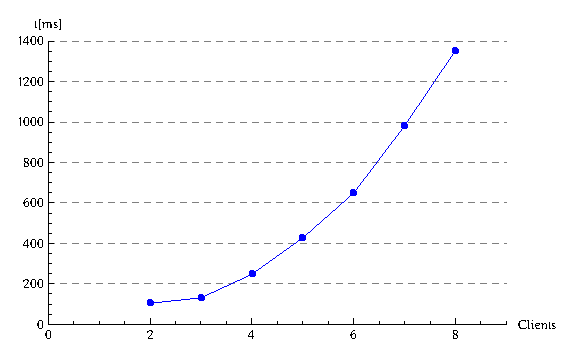
\includegraphics[width=\textwidth]{images_MessErgebnisse/incrementCacheSetBalance.eps}
\end{center}
\caption{\texttt{setBalance()}-Zeitaufwand, System mit Cache(nur schreibende Zugriffe)}
\end{figure}

Wenn alle beteiligten Clients schreibende Zugriffe tätigen, skaliert das System mit Cache sehr schlecht. 


In der nächsten Grafik wird die durchschnittliche Anzahl Konflikte pro Client gezeigt:
\begin{figure}[H]
\begin{center}
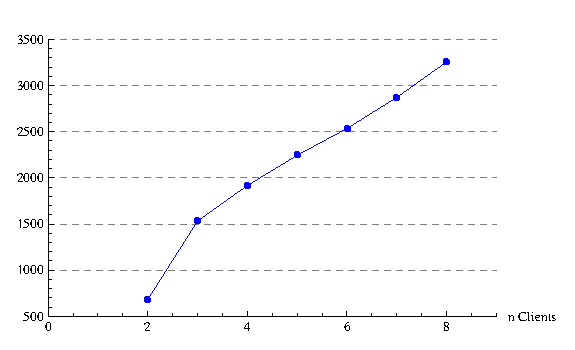
\includegraphics[width=\textwidth]{images_MessErgebnisse/incrementCacheKonfliktzahl.eps}
\end{center}
\caption{Anzahl Konflikte, System mit Cache(nur schreibende Zugriffe)}
\end{figure}

Die Anzahl der Konflikte nimmt linear mit der Anzahl Clients zu. Dies zeugt von einer schwachen Skalierbarkeit, da davon ausgegangen werden kann, dass diese Funktion linear weitersteigen würde, würden noch mehr Clients in den Test einbezogen.  

Pro zusätzlicher Client ergibt sich eine Zunahme der Konflikte um 250. Würde die Funktion analog weitersteigen, und davon ist auszugehen, würde die Anzahl Konflikte pro Client vermutlich auf über 6000 ansteigen, bei 20 Clients. Dennoch sollte bedacht werden, dass dieser Testcase ein Extrem darstellt, da jeder Client mit vollem Tempo zu schreiben versucht. 

Die Zeiten der \texttt{setBalance()}-Aufrufe steigen stark an, während die Anzahl der Konflikte nur linear steigt. Die Behandlung von 3000 Konflikten verursacht also eine ungemein höhere Zeitverzögerung, als dies 2000 Konflikte tun. 

Die nächste Grafik beschäftigt sich mit der reinen Durchführungszeit:
\begin{figure}[H]
\begin{center}
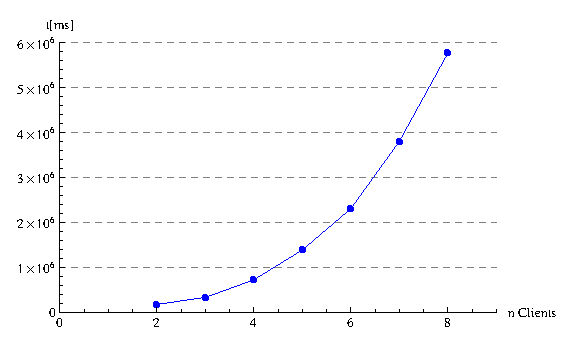
\includegraphics[width=\textwidth]{images_MessErgebnisse/incrementCachePureOperationTime.eps}
\end{center}
\caption{Pure Operation Time, System ohne Cache(nur schreibende Zugriffe)}
\end{figure}

Die starke Steigung dieser Funktion war durch die starke Steigung der \texttt{setBalance()}-Funktion abzusehen. Zwischen diesen zwei Grafiken besteht ein direkter Zusammenhang. Eine stark ansteigende \texttt{setBalance()}-Funktion führt unweigerlich zu einer stark ansteigenden Funktion der Durch\-führungs\-zeit. Da die \texttt{setBalance()}-Aufrufe mehr Zeit benötigen, wird der Testcase auch mehr Zeit in Anspruch nehmen.

\subsubsection{Interpretation}


Die \texttt{setBalance()}-Werte des System ohne Cache sind sehr stabil. Obwohl die \texttt{getBalance()}-Aufrufe gewohnt um einiges langsamer waren, als beim System mit Cache, konnte das System ohne Cache schlussendlich durch die stabilen Werte der \texttt{setBalance()}-Aufrufe die besseren Ergebnisse liefern.

Das Anzahl der Konflikte beim System mit Cache weisen an sich einen besseren Verlauf, als die Konfliktanzahl des Systems ohne Cache, aus. Da aber die \texttt{set\-Balance()}-Auf\-ru\-fe des Systems mit Cache viel schlechter skalierten, als die Werte des Systems ohne Cache, blieb der Performancevorteil aus. Insgesamt skaliert bei diesem Szenario das System ohne Cache um einiges besser.

Bei beiden Systemen treten sehr viele Konflikte auf, vor allem natürlich bei acht Clients. Bei einem solchen Einsatzszenario scheinen beide Systeme nicht ideal zu sein, da die Konfliktbewältigung viel Performance benötigt. Bei sehr vielen Schreibzugriffen, macht der Cache aber bei einer steigenden Anzahl Clients immer weniger Sinn, da die Geschwindigkeit der  \texttt{setBalance()}-Methode stetig abnehmen wird.

\section{Messerfahrungen}
Die Auswertung der Messdaten und deren Interpretation nahm sehr viel Zeit in Anspruch. Wie bereits im Kapitel \ref{sec:reportGenerator} "'Report Generator"' erläutert, hätte das Speichern der Resultate in einer anderen Art als Textdateien sehr viel weniger Zeit gekostet. Da die Resultate pro Szenario in einer einzelnen Textdatei vorhanden waren, mussten zusätzlich ein kleines Script geschrieben werden, welches  aus jedem Szenario die Zusammenfassungen liest und diese in einer gemeinsamen Datei abspeichert. Jedoch war der Aufwand für das Zusammenführen der Daten trotzdem extrem hoch, da die Daten manuell aus der Zusammenfassung nach Excel exportiert werden mussten. 

\paragraph{Start Script}
Zu Beginn der Messphase nutzte man das bereits vorhandene Start-Script für die einzelnen TestCases. Schon nach kurzer Zeit musste das Script jedoch so angepasst werden, dass es selbstständig alle Tests für einen Testcase ausführt. Das heisst, es skaliert den Test von zwei bis acht Clients selbstständig und führt dabei jeweils dreimal denselben Test durch, um einen verlässlichen Mittelwert pro Anzahl Clients ermitteln zu können.

\paragraph{Read Aktion}
Während des ersten Testlaufs des Szenarios, bei welchem ein Client schreibt und die restlichen nur lesen, stellte sich ein Problem mit dem Szenario Aufbau heraus. Die Idee dieses Szenarios liegt darin, dass die lesenden Clients solange aktiv gehalten werden, wie der schreibende Client Zeit benötigt für die Abarbeitung seines Szenarios. Das Problem war nun, dass die Clients bei der Cache Variante viel früher fertig waren und terminierten, dadurch konnte die gewünschte Interaktion zwischen den Clients nicht aufgezeigt werden. So blieb nur die Möglichkeit den Testcase anzupassen.
\begin{enumerate}
\item In einer ersten Variante wurde die Anzahl der Reads von 1'000 auf 1'000'000 vergrössert. Das Problem mit dieser Lösung war, dass das Szenario Objekt, welches auf dem Server für die einzelnen Clients erzeugt wurde, zu gross wurde und zu einem Heap Space Fehler führte. Eine Erhöhung des JVM Heap Space hätte das Problem ebenfalls nicht gelöst. Die Auswertung eines Clients hätte eine Datei mit über 1'000'000 Zeilen erzeugt. Diese Datei wäre enorm gross geworden und hätte die manuelle Auswertung extrem erschwert.   
\item Die Erkenntnis aus dem ersten Versuch führt dazu, dass die Read Aktion modifiziert werden musste. Wie bereits in der Increment Aktion wurde auch in der Read Aktion ein Delay eingebaut, der dabei helfen soll, die Dauer eines Szenarios vorhersagbar zu machen und das Szenario Objekt nicht zu gross werden lässt.
\end{enumerate}

\paragraph{Logger}
Bereits zu Beginn der Messungen kamen erste Zweifel hoch, über den Speicherplatzverbrauch der einzelne Testcases. Wie sich später herausstellte, lag der Grund für den grossen Speicherplatzverbrauch in der extrem grossen Logdatei, die vom Testframework Server generiert wurde. Die Datei wurde teilweise so gross, dass das Betriebssystem keinen Platz mehr für sich selber besass und den Testcase einfach beendet hat. Die Lösung lag in der Deaktivierung des Loggers in der Methode \verb+methodCalled()+. Was jedoch zur Folge hatte, das alle Messungen nochmals gemacht werden mussten, um eine Verfälschung der Daten auszuschliessen.

